\chapter{Equations Of Motion}
The dynamics of magnetic nozzle can be characterized by conservation of mass and momentum,
\begin{align*}
    &\pdv{n}{t} + B\pdv{z}(\frac{nv}{B}) = 0\\
    &\pdv{v}{t} + v\pdv{v}{z} = -c_s^2\frac{1}{n}\pdv{n}{z}
\end{align*}
Usually, the magnetic field can be described by
\[ B(z) = B_0\left[ 1 + R\exp(-\frac{z^2}{\delta^2}) \right] \]
where $R$ and $\delta$ are some coefficients.

At equilibrium (stationary solution), we have $\pdv*{n_0}{t}=0$ and $\pdv*{v_0}{t}=0$, so $n_0$ and $v_0$ satisfy
\begin{align*}
    &\pdv{z}(\frac{n_0v_0}{B}) = 0 \\
    &v_0\pdv{v_0}{z} = -c_s^2\frac{1}{n_0}\pdv{n_0}{z} 
\end{align*}
Let $M\equiv v_0/c_s$, then it can be represented by Lambert function, 
\[ M = \left[ -W\left(-M_m^2 \frac{B(z)^2}{B_m^2}e^{-M_m^2}\right) \right]^{1/2} \]
where $B_m\equiv 1+R$ is the maximum magnetic field (or magnetic field at mid-point), and $M_m$ is the mach number at mid-point. Below shows a few cases of the solution.
\begin{itemize}
    \item $M_m < 1$, subsonic velocity profile.
    \item $M_m = 1$, accelerating or decelerating profile (depending on the branch of the Lambert function).
    \item $M_m > 1$, supersonic velocity profile
\end{itemize}
\begin{figure}[H]
    \centering
    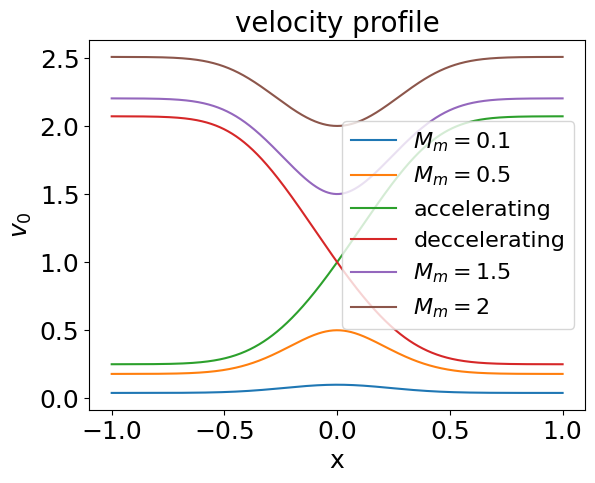
\includegraphics[width=0.7\linewidth]{img/nozzle-velocity-profile.png}
    \caption{$M_m < 1$, subsonic. $M_m = 1$, accelerating if we select Lambert function branch $k=0$ for $z<0$ and brach $k=-1$ for $z>=0$; decelerating if we choose branch $k=-1$ for $z<0$ and brach $k=0$ for $z>=0$. $M_m > 1$, supersonic.}
    \label{fig:nozzle-velocity-profile}
\end{figure}

For convenience, we nondimensionalize the equations by normalizing the velocity to $c_s$, $v\mapsto v/c_s$, $z$ to system length $L$, $z \mapsto z/L$ and time $t\mapsto c_s t/L$.
\begin{align}
    &\pdv{n}{t} + n\pdv{v}{z} + v\pdv{n}{z} - nv\frac{\partial_z B}{B} = 0 \\
    &n\pdv{v}{t} + nv\pdv{v}{z} = -\pdv{n}{z}
\end{align}
and the nondimensionalized equilibrium condition is
\begin{align}
    &\pdv{z}(\frac{n_0v_0}{B}) = 0 \label{eq:equilibrium-convervation-of-mass}\\
    &v_0\pdv{v_0}{z} = -\frac{1}{n_0}\pdv{n_0}{z} \label{eq:equilibrium-convervation-of-momentum}
\end{align}


\begin{proposition}
    Let $n = n_0(z) + \tilde{n}(z,t)$ and $v = v_0(z) + \tilde{v}(z,t)$, the linearized equations of motion are
    \begin{align}
        &\frac{1}{n_0}\pdv{\tilde{n}}{t} 
        + \pdv{\tilde{v}}{z} + v_0\tilde{Y} + \tilde{v}\frac{\partial_z n_0}{n_0} - \tilde{v}\frac{\partial_z B}{B} = 0 
        \label{eq:linearized-conservation-of-mass}
        \\
        &\pdv{\tilde{v}}{t} + \pdv{(v_0\tilde{v})}{z} = -\tilde{Y}
        \label{eq:linearized-conservation-of-momentum}
    \end{align}
    where 
    \[ \tilde{Y} \equiv \frac{1}{n_0}\pdv{\tilde{n}}{z} - \frac{\partial_z n_0}{n_0^2}\tilde{n} = \pdv{z}(\frac{\tilde{n}}{n_0}) \]
\end{proposition}
\begin{proof}
    We first derive Eq.(\ref{eq:linearized-conservation-of-mass}). We linearize Eq.(\ref{eq:equilibrium-convervation-of-mass}) by setting $n=n_0+\tilde{n}$ and $v=v_0+\tilde{v}$. By ignoring the second order perturbations, we obtain
    \begin{align*}
        &\pdv{(n_0+\tilde{n})}{t} 
        + (n_0+\tilde{n})\pdv{(v_0+\tilde{v})}{z} 
        + (v_0+\tilde{v})\pdv{(n_0+\tilde{n})}{z} 
        - (n_0+\tilde{n})(v_0+\tilde{v})\frac{\partial_z B}{B} = 0 \\
        \Rightarrow 
        &\pdv{\tilde{n}}{t} 
        + n_0\pdv{v_0}{z} + \tilde{n}\pdv{v_0}{z} + n_0\pdv{\tilde{v}}{z}
        + v_0\pdv{n_0}{z} + \tilde{v}\pdv{n_0}{z} + v_0\pdv{\tilde{n}}{z} 
        - (n_0v_0 + n_0\tilde{v} + \tilde{n}v_0)\frac{\partial_z B}{B} = 0 \\
        \Rightarrow
        &\frac{1}{n_0}\pdv{\tilde{n}}{t} 
        + \pdv{v_0}{z} + \frac{\tilde{n}}{n_0}\pdv{v_0}{z} + \pdv{\tilde{v}}{z}
        + \frac{v_0}{n_0}\pdv{n_0}{z} + \frac{\tilde{v}}{n_0}\pdv{n_0}{z} + \frac{v_0}{n_0}\pdv{\tilde{n}}{z} 
        - v_0\frac{\partial_z B}{B} - \tilde{v}\frac{\partial_z B}{B} - \tilde{n}\frac{v_0}{n_0}\frac{\partial_z B}{B} = 0
    \end{align*}
    Using the equilibrium condition Eq.(\ref{eq:equilibrium-convervation-of-mass}), some of the terms are canceled and the last term can be written as 
    \[ \tilde{n}\frac{v_0}{n_0}\frac{\partial_z B}{B} = \frac{\tilde{n}}{n_0}\left( \frac{\partial_z n_0}{n_0}v_0 + \pdv{v_0}{z} \right) \]
    Now, we are left with equation
    \[
        \frac{1}{n_0}\pdv{\tilde{n}}{t}
        + \pdv{\tilde{v}}{z}
        + v_0\underbrace{\left(\frac{1}{n_0}\pdv{\tilde{n}}{z} - \frac{\tilde{n}}{n_0}\frac{\partial_z n_0}{n_0}  \right)}_{\tilde{Y}}
        + \frac{\tilde{v}}{n_0}\pdv{n_0}{z}
        - \tilde{v}\frac{\partial_z B}{B} = 0
    \]

    To derive Eq.(\ref{eq:linearized-conservation-of-momentum}), we linearize the LHS of the conservation of momemtum
    \begin{align*}
        &(n_0+\tilde{n})\pdv{(v_0+\tilde{v})}{t} + (n_0+\tilde{n})(v_0+\tilde{v})\pdv{(v_0+\tilde{v})}{z} = -\pdv{n}{z} \\
        \Rightarrow 
        & \pdv{v_0}{t} + \frac{\tilde{n}}{n_0}\pdv{v_0}{t} + \pdv{\tilde{v}}{t} 
        + \left(v_0+\tilde{v}+\frac{\tilde{n}}{n_0}v_0\right)\pdv{(v_0+\tilde{v})}{z} = -\frac{1}{n_0}\pdv{n}{z}\\
        \Rightarrow
        & \pdv{v_0}{t} + v_0\pdv{v_0}{z} + \tilde{v}\pdv{v_0}{z} 
        = -\frac{1}{n_0}\pdv{n_0}{z} -\frac{1}{n_0}\pdv{\tilde{n}}{z} -v_0\frac{v_0}{z} - \frac{\tilde{n}}{n_0}v_0\pdv{v_0}{z} \\ 
    \end{align*}
    Using the equilibrium condition Eq.(\ref{eq:equilibrium-convervation-of-momentum}) on the RHS, we get the desired form.
\end{proof}

\[ \int fdx = 1 \]

\cite{stellingwerf_stability_1978}